%************************************************
\chapter{The Simulation}
\label{chapter:the_simulation}
%************************************************

It is imperative to understand that the \emph{simulation model} is not
the same as the model of mind that was previously described.  The
simulation model is an extension of the model of mind that includes a
mathematical description of a discrete ``state'' of the model in a
discrete time.  Neither the model of mind nor the simulation model
changes over time.  The simulation model therefore includes a
discretely stepped state that is used to simulate the necessarily
separate, static model of mind.  The term ``simulation'' is thus used
as a general reference to the dynamic activity in Duration that
manipulates and steps the state of the simulation model.  In
describing the simulation model, it is important to not confuse the
dynamic activity of simulation with the model or the state of the
model, which are both static at any given point in time.  The term
``simulation'' is the only reference to activities in Duration.  This
distinction is necessary for the simulation model to not be limited to
simulating a specific kind of activity.

For example, consider a simulation of topological proof.  A
mathematician can ``simulate'' the rules of topological proof by first
seeing a static arrangement of symbols on paper.  These symbols can be
manipulated in the process of proving or disproving the initial
topological statement.  There is no existing logical or mathematical
formulation of the activities of topological proof.  I describe how a
symbolic state space can be added to the model of mind for the
purposes of simulation.  How exactly this simulation is done is left
until the next part, where the activity of simulation is assumed to be
computational.

The activities in Duration in the model of mind exist prior to their
symbolization, and since it is obviously not possible to refer to
something prior to symbolizing it, the assumption that these
activities have already been symbolized is necessary in order to
mathematically describe the state of the simulation model.  Defining
the simulation model requires a description in terms of symbols for
the ``undescribed activities in Duration.''  Each assumption made in
symbolizing the ongoing activities in Duration restricts the
simulation model from being a model of those assumptions because only
the symbolic result of those assumptions is available for the
simulation of the activity of reflection.

\section{Representing Dynamic Activities as a Set}

\begin{figure}
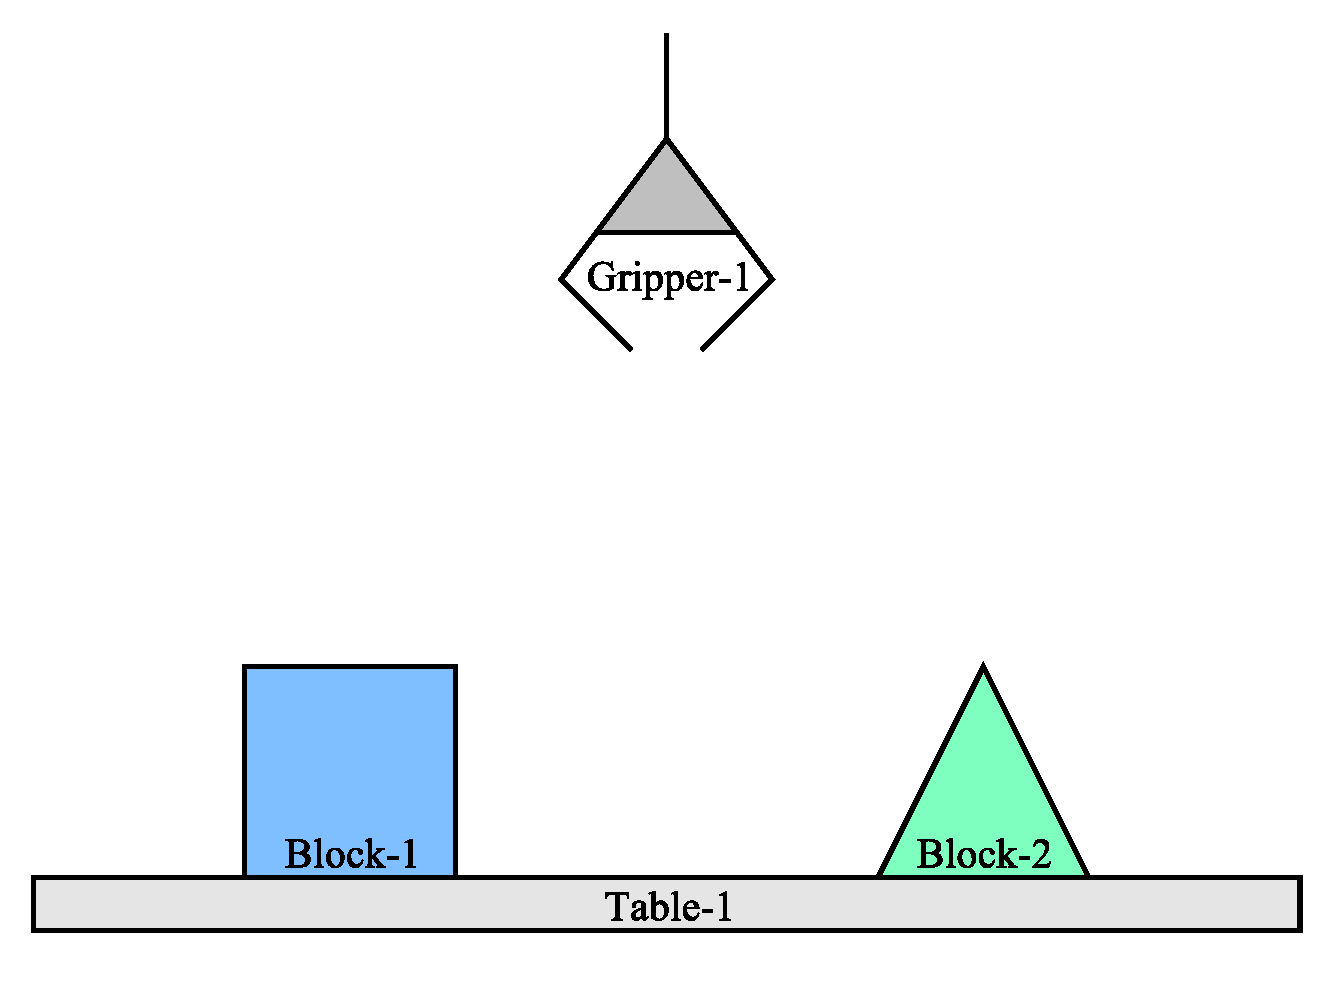
\includegraphics[width=10cm]{gfx/blocks_world_simulation}
\caption{An example for simulation.}
\label{figure:blocks_world_simulation}
\end{figure}

I will begin with one of the simplest mathematical models, a
\emph{set} of symbols, to model of the activities in Duration.  I will
first describe the simulation model as the mathematical set, $S$, the
state.  Here is an example of a possible symbolization of the
activities shown in {\mbox{\autoref{figure:blocks_world_simulation}}}:
\begin{equation}
\label{equation:example_initial_state}
S =
  \left\{
    \begin{array}{l}
      \text{{\tt{Gripper-1}}}, \\
      \text{{\tt{Block-1}}}, \\
      \text{{\tt{Block-2}}}, \\
      \text{{\tt{Table-1}}}
    \end{array}
  \right\}
\end{equation}
At any given point in the simulation, the state, $S$, is static, but
the simulation can have different static states at different time
steps, $n$, giving a number of static states, $S[n]$.  The simulation
process is a discrete stepwise activity.  The simulation step is the
dynamic activity that is not part of the state, $S$, of the simulation
model.  I will now describe a notation for referring to the different
states that result from a simulation process.

\section{Simulation States}

Equations~\ref{equation:simulate_first}
and~\ref{equation:simulate_last} show a notation for referring to the
state of a simulation after a number of simulation steps, $n$.
\begin{align}
\label{equation:simulate_first}
S[0] &= \text{\emph{The Initial State}} \\
\label{equation:simulate_last}
S[n] &= \text{\emph{simulate}}~S[n-1]
\end{align}
Equation~\ref{equation:simulate_first} defines $S[0]$ to be
the initial representation of the activities in Duration that are
being simulated; an example of the initial state was given previously
in Equation~\ref{equation:example_initial_state}.
Equation~\ref{equation:simulate_last} introduces an explicit reference
to the activity of simulation with the symbol ``simulate.''  Because I
have not yet defined this activity, these equations still have a
reference to the actual dynamic activity of simulation.  I use this
notation to discuss how the state, $S$, changes during the
actual process of simulation.  I will use the notation in
Equation~\ref{equation:simulate_n_steps} to refer to the state of the
simulation after $n$ actual steps of simulation activity:
\begin{equation}
\label{equation:simulate_n_steps}
S[n] = \text{\emph{simulate}}^n~S[0]
\end{equation}

\section{Representing Continuous Space as a Set of 3-Tuples}

The activities in Duration are symbolized in the layer above, while
these symbolic activities are in different actively ordered Spatial
relationships, which can also be symbolized by the layer above.  I
will use a 3-tuple to represent the activity of a Spatial relationship
in the simulation.  Reconsidering the activities shown in
{\mbox{\autoref{figure:blocks_world_simulation}}}, the state could be
represented by the set of 3-tuples shown in
{\mbox{\autoref{equation:example_stricly_ordered_set_initial_state}}}.
\begin{equation}
\label{equation:example_stricly_ordered_set_initial_state}
S =
  \left\{
    \begin{array}{l}
      (\text{\tt{Block-1}},   ~\text{\tt{sitting-on}},  ~\text{\tt{Table-1}}), \\
      (\text{\tt{Block-2}},   ~\text{\tt{sitting-on}},  ~\text{\tt{Table-1}}), \\
      (\text{\tt{Gripper-1}}, ~\text{\tt{being-above}}, ~\text{\tt{Table-1}}), \\
      (\text{\tt{Gripper-1}}, ~\text{\tt{moving}},      ~\text{\tt{left}})
    \end{array}
  \right\}
\end{equation}

\section{Defining a Graph}

A set of 3-tuples can be thought of as a graph with labelled nodes and
edges.  Because the graph provides a clear notation for referring to
types of Spatial arrangements of activities, the notation of
{\mbox{\cite{messmer:1995}}} is used to define a labelled graph in
{\mbox{Definition~\ref{definition:graph_first}}} and a labelled
subgraph in {\mbox{Definition~\ref{definition:graph_last}}}.

\begin{definition}
\label{definition:graph_first}
\emph{
A graph $G$ is the 4-tuple $(V, ~e, ~\mu, ~\nu)$, where
\begin{itemize}
\item $V$ is the set of vertices,
\item $E ~{\subseteq}~ V ~{\times}~ V$ is the set of edges,
\item $\mu : V \mapsto \ell_V$ is a function assigning labels to the vertices,
\item $\nu : E \mapsto \ell_E$ is a function assigning labels to the edges.
\end{itemize}
}\end{definition} \noindent In this definition, the edges are
directed, i.e. there is an edge from $v_1$ to $v_2$ if
$(v_1,v_2){\in}E$.  The empty graph, i.e. the graph with an empty set
of vertices will be denoted by $\emptyset$.

\begin{definition}
\label{definition:graph_last}
\emph{
Given a graph $G = (V, e, \mu, \nu)$, a \emph{subgraph} of $G$ is a
graph $G_s = (V_s, e_s, \mu_s, \nu_s)$ such that
\begin{enumerate}
\item $V_s {\subseteq} V$
\item $E_s = E \cap (V_s {\times} V_s)$
\item $\mu_s$ and $\nu_s$ are the restrictions of $\mu$ and $\nu$ respectively, i.e.
\begin{align*}
\mu_s(v) &= {\left\{
               \begin{array}{ll}
                 \mu(v)           & \text{if }v {\in} V_s \\
                 \text{undefined} & \text{otherwise}
               \end{array}
             \right.} \\
\nu_s(e) &= {\left\{
               \begin{array}{ll}
                 \nu(e)           & \text{if }e {\in} E_s \\
                 \text{undefined} & \text{otherwise}
               \end{array}
             \right.}
\end{align*}
\end{enumerate}
}\end{definition} \noindent From this definition it is easy to see
that, given a graph $G$, any subset of its vertices each uniquely
defines a subgraph of $G$.  The notation $G_s ~{\subseteq}~ G$ is used
to indicate that $G_s$ is a subgraph of $G$.

\section{Representing Continuous Space as a Graph}

\begin{figure}
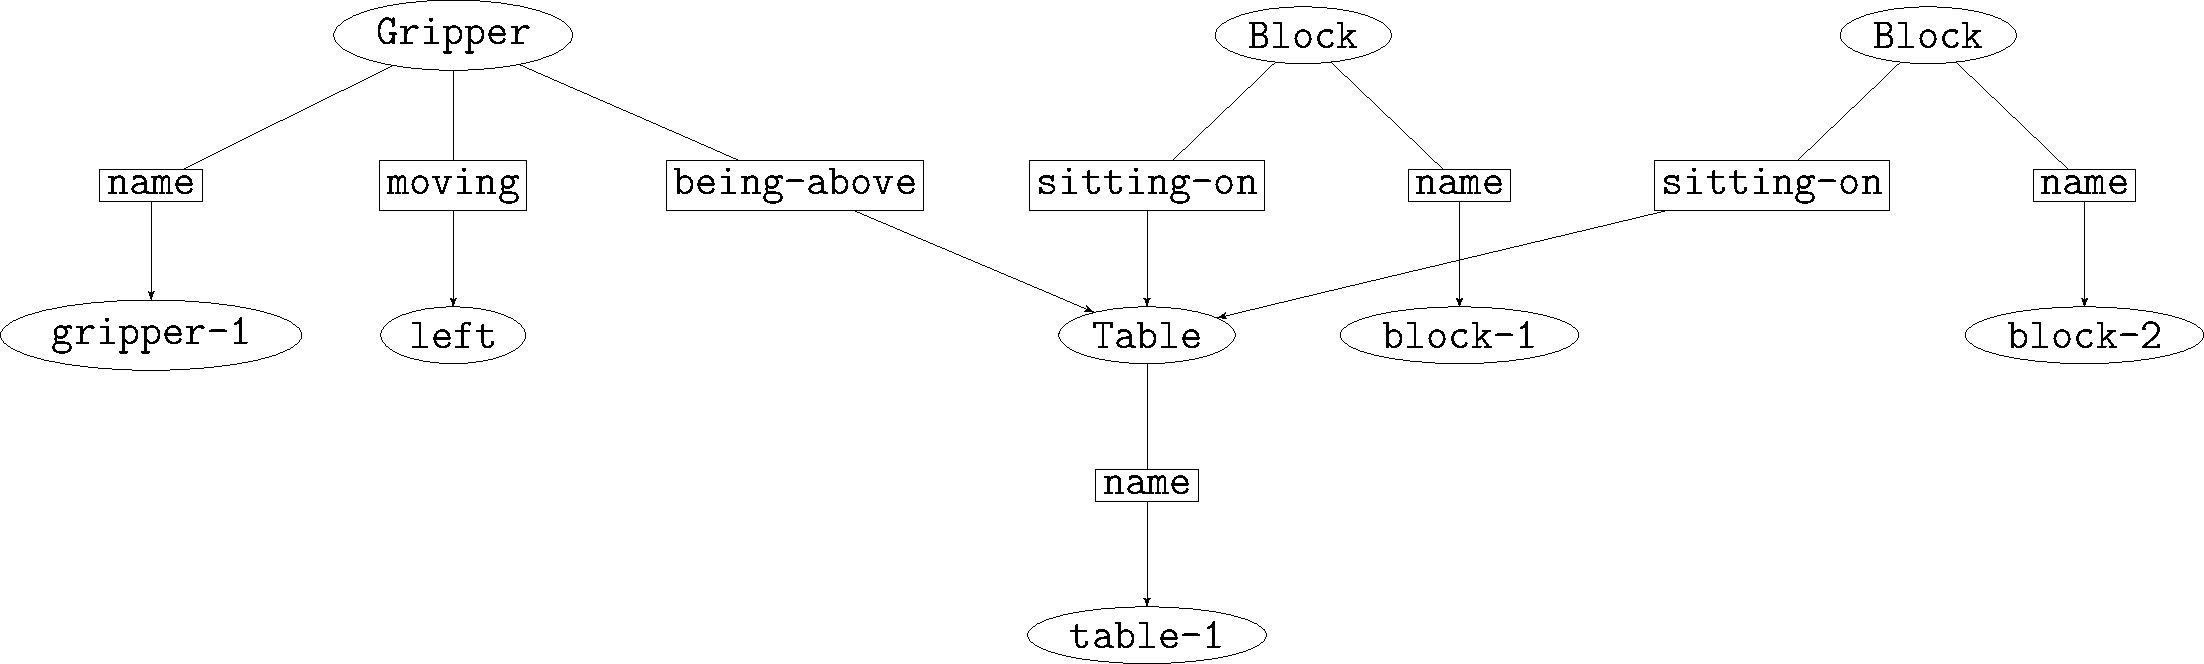
\includegraphics[width=10cm]{gfx/simulation_example_state}
\caption{A graph representation of a state space.}
\label{figure:simulation_example_state}
\end{figure}

%\begin{definition}\emph{

%}\end{definition}


%\section{The Mistake of Including Dynamic Activity in the Simulation Model}



\section{Symbols and Simulated Symbols}

It becomes important at this point to keep track of the layer of
modelling that results when one simulates thinking.  Therefore, I will
use an asterisk notation for referring to different classes of
simulated modelling.  For example, I will continue to use, simply, the
term symbol to refer to the symbols that have actually been
reflectively symbolized in order to refer to the activities in
Duration.  When I am referring to the simulation of the process of
symbolization, I will refer to this as a simulated symbol, or a
\emph{symbol*}.  A symbol* is a simulated symbol that is created by
the simulation.  The symbol* is a static reference that is simulated
as being grounded in the symbols in the simulation state, the
simulated activities in Duration.

\section{Representing Existence}

Activities actually exist.  Once we have considered the activities in
Duration to be the set of symbols, $S$, we have assumed static
representations for the actual dynamic.  The dynamic does not have
terms to help us in representing.  Therefore, the question of
existence becomes a question of whether or not a symbol is in the set
that is the current state of the simulation, $S$.
Equation~\ref{equation:exists} shows a definition of {\tt exists}, a
logical relationship between any symbolic reference to activity
contained in the simulation state:
\begin{equation}
\label{equation:exists}
\text{exists}(x) \longleftrightarrow x{\in}S, \text{ ~~~for all }x{\in}S
\end{equation}

\section{Representing Symbolization}

In order to describe symbolization, a representation for a simulated
symbol must be defined.  A simulated symbol is actively maintained in
Duration, so the existence of a simulated symbol in the simulation
model would need to be added to the set of all simulated activities in
Duration.  The symbol*, $x^*$, has a referent, $\text{referent}(x^*)$,
a subset of the simulated activities in Duration, $S$, in
Equations~\ref{equation:symbolization_first}
and~\ref{equation:symbolization_last}:
\begin{align}
\label{equation:symbolization_first}
                 x^* &= \text{\emph{Simulated Symbol}} \\
\text{referent}(x^*) &\subseteq S
\label{equation:symbolization_last}
\end{align}

%Equation~\ref{equation:existence_of_symbol} defines the relationship
%between the existence of a simulated symbol, $\text{exists}(x^*)$, the
%simulation state, $S$, and the simulated referent,
%$\text{referent}(x^*)$.
%This equation shows that if any symbol that
%is contained within the simulated referent set is in the simulation
%state, the symbol* is perceived:
%\begin{equation}
%\label{equation:existence_of_symbol}
%\text{perception(x^*) ~\longleftrightarrow~ (S ~{\cap}~ \text{referent}(x^*)) \neq \emptyset
%\end{equation}

\section{Tautological Symbolic Reference}

Consider the following definition, which defines a symbol* to
tautologically reference its own symbolization activity.
Equation~\ref{equation:tautological_reference} defines a tautological
referent for a symbol*, $x^*$:
\begin{equation}
\label{equation:tautological_reference}
x^* \in \text{referent}(x^*)
\end{equation}
Tautological references are meaningless, except if they are considered
reflectively to be a type of knowledge to manipulate.  In a model that
is symbolizing and perceiving the world in terms of symbols,
tautological symbolic references always have the potential for being
active perceptions because the existence of the symbol implies that
its referent, itself, is active.  When symbols are used for
perception, tautological references are at best distracting and at
worst render a model meaningless.

Because a tautological reference, like that in
Equation~\ref{equation:tautological_reference}, removes all utility
from symbols* in the simulation model, it is important that avoiding
tautological references is the default behavior.  In order to easily
avoid tautological references, I define an ordering for symbolic
references that keeps references from ever becoming purely
tautological.

\section{Sets of Symbol Activities}

Symbols are the static counterpart to the dynamic in the model of
mind.  Keeping track of which activities are simulations of dynamic
activity and which are simulations of static symbols, symbols*, is
critical for avoiding the creation of a tautological model with
symbols* only referring to other symbols*.
Equations~\ref{equation:symbol_activities_set_first}
and~\ref{equation:symbol_activities_set_last} define the set of
activities that are symbolic references:
\begin{align}
\label{equation:symbol_activities_set_first}
X^*_i &= \text{\emph{Symbol activities in reflective}}^i\text{\emph{ layer}} \\
\label{equation:symbol_activities_set_last}
X^*_i &\subseteq L_i
\end{align}

\section{Layers of Sets of Dynamic Activity}

In order to avoid tautological symbolic references, I have divided the
model into layers that order symbolic activities and references.  To
simulate the $\text{reflective}^n$ layers of activity in the model, I
must divide the simulation state, $S$, into reflective layers.
Equations~\ref{equation:layers_of_sets_first}
through~\ref{equation:layers_of_sets_last} give a definition of the
disjoint set of layers, $\mathbf{L}$, stating that the union of all
layers of activity is equal to the simulation state, $S$:
\begin{align}
\label{equation:layers_of_sets_first}
                            L_i &= \text{\emph{Activities of the} }\text{reflective}^i\text{ \emph{layer}} \\
                     \mathbf{L} &= \{L_0, ~L_1, ~L_2, ~...~ \} \\
\label{equation:layers_are_mututally_exclusive}
\forall_{A,B{\in}{\mathbf{L}}} ~ (A &= B ~{\vee}~ A{\cup}B = {\emptyset}) \\
\label{equation:layers_of_sets_last}
                      S &= \bigcup_{A{\in}\mathbf{L}}{A}
\end{align}
{\mbox{\autoref{equation:layers_are_mututally_exclusive}}} defines the
mutual exclusivity of layer activities.  Using these reflective layer
definitions, I define an ordering of symbol* references that prevents
symbols from every having tautological references.
Equation~\ref{equation:layered_symbol_references} defines that a
symbol may only refer to activities in the layers below its own layer
of activity:
\begin{equation}
\label{equation:layered_symbol_references}
x^* \in L_i \rightarrow \text{referent}(x^*) \subseteq \bigcup_{k=0}^{i-1}{L_k}
\end{equation}

\section{No Symbols* in Layer Zero}

Equations~\ref{equation:no_symbols_in_layer_zero_first}
through~\ref{equation:no_symbols_in_layer_zero_last} derive that a
symbol* cannot actively exist in the simulated reflective layer zero,
$L_0$.  Equation~\ref{equation:no_symbols_in_layer_zero_first} derives
from the layered symbolic references equation,
Equation~\ref{equation:layered_symbol_references}.
Equation~\ref{equation:no_symbols_in_layer_zero_exists} derives from
incorporating a reversed version of the symbol existence equation,
Equation~\ref{equation:existence_of_symbol}:
\begin{align}
\label{equation:no_symbols_in_layer_zero_first}
       x^* \in L_0 \rightarrow \text{referent}(x^*) &\subseteq \emptyset \\
\text{\emph{True}} \rightarrow \text{referent}(x^*) &= \emptyset \\
                               \text{referent}(x^*) &= \emptyset \\
\label{equation:no_symbols_in_layer_zero_exists}
\text{exists}(x^*) &\longleftrightarrow (S ~{\cap}~ \emptyset) \neq \emptyset \\
\text{exists}(x^*) &\longleftrightarrow \emptyset \neq \emptyset \\
\text{exists}(x^*) &\longleftrightarrow \text{\emph{False}}
\label{equation:no_symbols_in_layer_zero_last}
\end{align}

\section{Representing Space}

The activity of maintaining a Spatial relationship, $r_i$, occurs in
the $\text{reflective}^i$ layer.  Spatial relationships are able to
arrange any symbol* that exists in the layer
above, the set $X_{i+1}^*$.
Equations~\ref{equation:define_space_activity_first}
through~\ref{equation:define_space_activity_that} define how symbols
are Spatially arranged, $r_i$, from the layer below:
\begin{align}
\label{equation:define_space_activity_first}
                      r_i &= \text{\emph{Spatial relationship activity in} reflective}^i\text{\emph{ layer}} \\
                      r_i &\in L_i \\
\label{equation:define_space_activity_this}
         \text{this}(r_i) &\in X_{i+1}^* \\
\label{equation:define_space_activity_relation_type}
\text{relation-type}(r_i) &\in X_{i+1}^* \\
\label{equation:define_space_activity_that}
         \text{that}(r_i) &\in X_{i+1}^*
\end{align}
Equations~\ref{equation:define_space_activity_left}
and~\ref{equation:define_space_activity_right} define the {\tt left}
and {\tt right} symbolic referents of the $r_i$ simulated Spatial
relationship.  Note that the simulated Spatial arrangement activity is
in the layer below the symbols* that are being arranged.

Spatial relationships can refer to other Spatial relationships from
the same layer because the activity of the Spatial relationship is in
the layer below the symbols that it arranges, so one arrangement can
be symbolized and referred to by another arrangement from the same
layer.

The {\tt left} and {\tt right} symbolic* referents of the simulated
relationship are modelled after the ``cons'' cell of a Lisp program.
A two-part relationship that can be symbolized and put into other
two-part relationships is enough representation to write the entire
Lisp programming language.  So, the simulated relationship, $r_i$,
allows for representing any relational computer science object in this
sense.

\section{Representing the Transition}

Equations~\ref{equation:define_transition_activity_first}
through~\ref{equation:define_transition_activity_future} define a
transition, $t_i$:
\begin{align}
\label{equation:define_transition_activity_first}
               t_i &= \text{\emph{Transition activity in the} reflective}^i\text{\emph{ layer}} \\
               t_i &\in L_i \\
\label{equation:define_transition_activity_past}
  \text{past}(t_i, n) &\in X_{i+1}^* \\
\label{equation:define_transition_activity_future}
\text{future}(t_i, n) &\in X_{i+1}^*
\end{align}

\section{Representing the Hypothesis}

Equations~\ref{equation:define_hypothesis_activity_first}
through~\ref{equation:define_hypothesis_activity_result} define a
hypothesis, $h_i$:
\begin{align}
\label{equation:define_hypothesis_activity_first}
                  h_i &= \text{\emph{Hypothesis activity in the} reflective}^i\text{\emph{ layer}} \\
                  h_i &\in L_i \\
\label{equation:define_hypothesis_activity_cause}
    \text{cause}(h_i) &\in X_{i+1}^* \\
\label{equation:define_hypothesis_activity_necessity}
\text{necessity}(h_i) &\in X_{i+1}^* \\
\label{equation:define_hypothesis_activity_result}
   \text{result}(h_i) &\in X_{i+1}^*
\end{align}

\section{Representing Existence and Non-existence}

When the $\text{reflective}^1$ layer symbolizes physical activities, a
causal hypothesis can be created in the $\text{reflective}^2$ layer
that puts a reference to the ``non-existence'' of the symbol activity
in the past slot and the ``existence'' of the symbol in the future
slot.  The present cause can be any of the current activities in
either the $\text{reflective}^0$ or $\text{reflective}^1$ layers.
{\mbox{Equations~\ref{equation:define_creation_activity_first}}}
{\mbox{through~\ref{equation:define_creation_activity_existence}}}
show a representation for the simulation of the creation activity that
creates the existence of an activity in the layer below from the
``non-existence'' of the activity.
\begin{align}
\label{equation:define_creation_activity_first}
                      c_i &= \text{\emph{Creation activity in the} reflective}^i\text{\emph{ layer}} \\
                      c_i &\in L_i \\
\label{equation:define_creation_activity_cause}
        \text{cause}(c_i) &\in X_{i+1}^* \\
\label{equation:define_creation_activity_non_existence}
\text{non-existence}(c_i) &\in X_{i+1}^* \\
\label{equation:define_creation_activity_existence}
    \text{existence}(c_i) &\in X_{i+1}^*
\end{align}

\section{Representing Knowledge of Symbolic Existence}


\section{Simulating Goals}

Activities in Duration can be symbolized as goals.  The symbolization
of a goal in the $\text{reflective}^i$ layer can be simulated by the
symbolic simulated activity, $g_i$.

\section{leftovers...}

\section{Simulating the Transframe}

Equations~\ref{equation:define_transframe_activity_first}
through~\ref{equation:define_transframe_activity_remove} define a
transframe, $\text{trans}_i$:
\begin{align}
\label{equation:define_transframe_activity_first}
                  \text{trans}_i &= \text{\emph{Transframe activity in the} reflective}^i\text{\emph{ layer}} \\
                  \text{trans}_i &\in L_i \\
\label{equation:define_transframe_activity_add}
   \text{add}(\text{trans}_i) &\in X_{i+1}^* \\
\label{equation:define_transframe_activity_remove}
\text{remove}(\text{trans}_i) &\in X_{i+1}^*
\end{align}

%\section{Simulating the Plan}
%


%\section{State Transitions (should be rewritten in simulation objects)} 

%\autoref{figure:blocks_world_gripper_over_block} shows an example of
%the next state of the simulation, $S[1]$.
%Equation~\ref{equation:example_next_state} gives an example
%description of the next state of the simulation model:
%\begin{figure}[bth]
%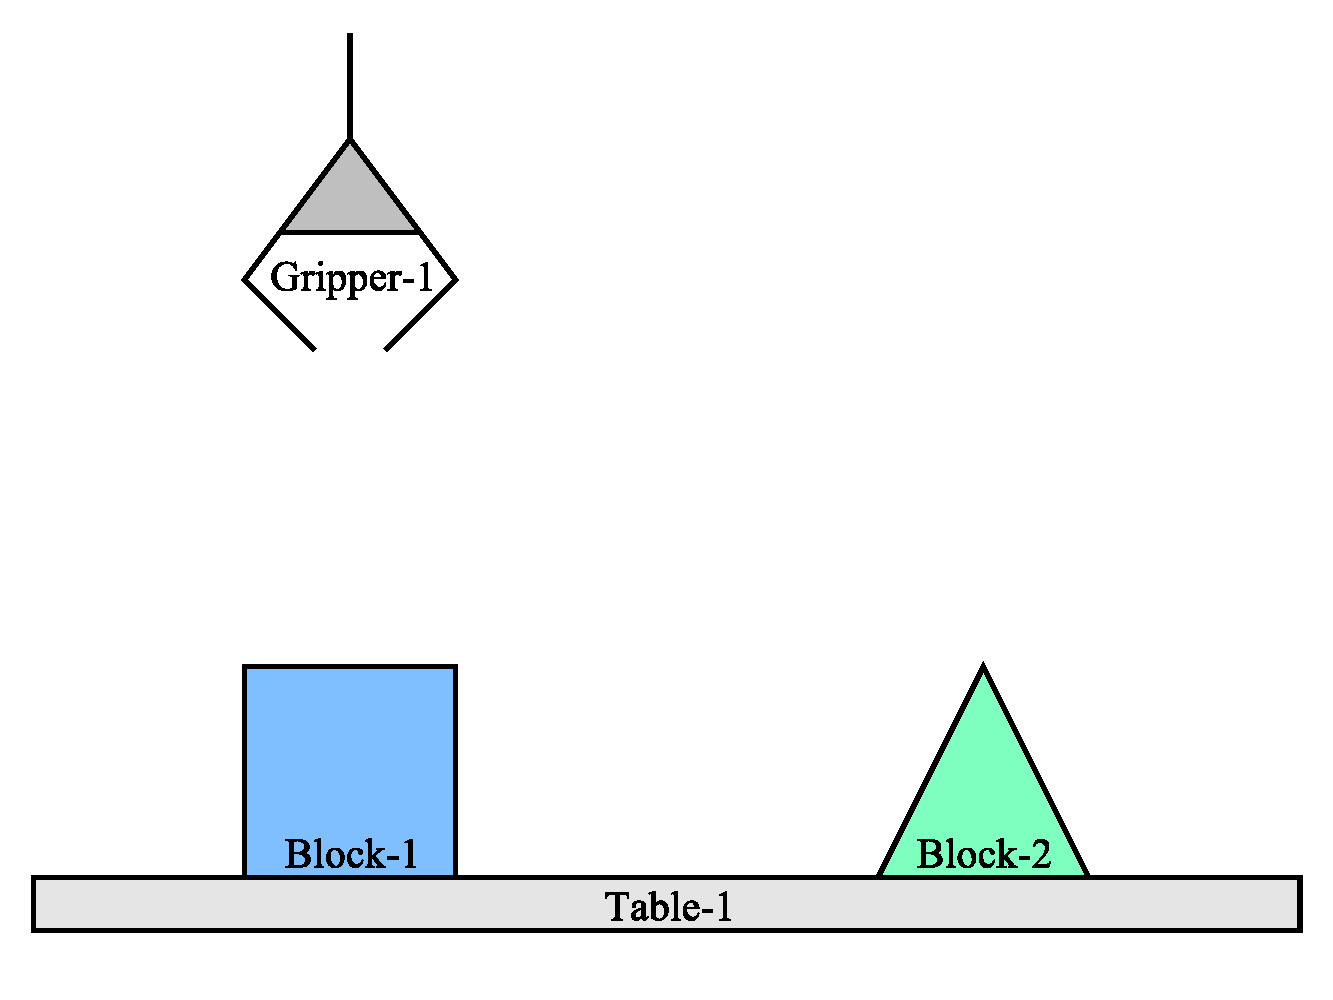
\includegraphics[width=10cm]{gfx/blocks_world_gripper_over_block}
%\caption{An example future state of simulation.}
%\label{figure:blocks_world_gripper_over_block}
%\end{figure}
%\begin{equation}
%\label{equation:example_next_state}
%S[1] =
%  \left\{
%    \begin{array}{l}
%      \text{{\tt Block-1-sitting-on-Table-1}}, \\
%      \text{{\tt Block-2-sitting-on-Table-1}}, \\
%      \text{{\tt Gripper-1-hovering-above-Table-1}}, \\
%      \text{{\tt Gripper-1-hovering-above-Block-1}}
%    \end{array}
%  \right\}
%\end{equation}
%
%Now, in order to begin to describe the activity of simulation, we must
%explicitly represent the transition, $T$, from one state to another.
%I refer to the resulting change to the state of the simulation as a
%\emph{state transition}.  The transition, $T[n]$, consists of two sets
%that keep track of changes, the \emph{add} set and the \emph{remove}
%set, as shown in Equation~\ref{equation:state_transition}:
%\begin{equation}
%\label{equation:state_transition}
%T[n] = \{T_\text{add}[n], ~T_\text{remove}[n]\}
%\end{equation}
%Equations~\ref{equation:predictive_state_transition}
%through~\ref{equation:transframe_last} give a definition of the
%transition, $T[n]$, in terms of the states, $S[n]$ and
%$S[n+1]$:
%\begin{align}
%\label{equation:predictive_state_transition}
%          S[n+1] & = S[n] ~{\cup}~ T_\text{add}[n] ~{\setminus}~ T_\text{remove}[n] \\
%         T_\text{remove}[n] & ~{\subseteq}~ S[n] \\
%         T_\text{remove}[n] & ~{\not\subseteq}~ S[n+1] \\
%            T_\text{add}[n] & ~{\subseteq}~ S[n+1] \\
%\label{equation:transframe_last}
%            T_\text{add}[n] & ~{\not\subseteq}~ S[n]
%\end{align}
%Equations~\ref{equation:state_transition_first}
%and~\ref{equation:state_transition_last} give the state transition,
%$T[n]$, for every step of the simulation:
%\begin{align}
%  \label{equation:state_transition_first}
%     T_\text{add}[n] &= S[n+1] ~{\setminus}~ S[n] \\
%  \label{equation:state_transition_last}
%  T_\text{remove}[n] &= S[n]   ~{\setminus}~ S[n+1]
%\end{align}
%Equation~\ref{equation:predictive_state_transition} shows the
%predictive potential for knowing the transition, $T[n]$, given the
%current state, $S[n]$.  Of course, $T[n]$ is defined in
%terms of $S[n]$ \emph{and} $S[n+1]$, so any
%predictive potential for
%Equation~\ref{equation:predictive_state_transition} is purely
%hypothetical.

